\begin{uebung}[1]
	\begin{aufgabe}
		Diskutieren Sie ohne Ableitung.

		\[
			y = \frac{x^3}{{(x-1)}^2}
		\]
	\end{aufgabe}

	\begin{loesung}

		\subparagraph{Nullstellen}
		Dreifache Nullstelle bei \(x = 0 \Rightarrow \) Sattelpunkt

		\subparagraph{Polstelle}
		Zweifache Polstelle bei \(x = 1 \Rightarrow \) PS ohne Vorzeichenwechsel

		\subparagraph{Symmetrie}
		weder gerade noch ungerade: nicht symmetrisch

		\subparagraph{Polynomdivision}
		\polyset{style=C, div=:,vars=x}
		\polylongdiv{x^3}{x^2 -2x + 1}

		\[
			y = \underbrace{x + 2}_{\text{\color{cyan}Asymptote}} + \underbrace{\frac{3x - 2}{{(x - 1)}^2}}_{\text{echt gebrochen}}
		\]

		\begin{figure}[H]
			\centering
			\begin{tikzpicture}
				\begin{axis}[
						default,
						xmin=-8.2, xmax=8.2,
						ymin=-8.2, ymax=8.2,
						width=8cm
					]
					\draw [orange, smooth, samples=100, domain=-8.2:0.9] plot (\x, {pow(\x, 3) / pow((\x - 1), 2)});
					\draw [orange, smooth, samples=100, domain=1.1:8.2] plot (\x, {pow(\x, 3) / pow((\x - 1), 2)});
					\draw [dashed, cyan, samples=100, domain=-8.2:8.2] plot (\x, {\x+2});
					\draw[dashed, gray] (1, -8.2) -- (1, 8.2);
				\end{axis}
			\end{tikzpicture}
			\caption{Skizze}
		\end{figure}
	\end{loesung}
\end{uebung}

\begin{uebung}[2]
	\begin{aufgabe}
		Diskutieren Sie ohne Ableitung.

		\[
			y = x^3 + x^2 - 8x - 12
		\]
	\end{aufgabe}

	\begin{loesung}

		\subparagraph{Nullstellen}
		1. Nullstelle raten: \(x_{N1} = 3\)

		\polyset{style=C, div=:,vars=x}
		\polylongdiv{x^3 + x^2 -8x -12}{x -3}

		2./3. Nullstelle bei \(x_{N2} = -2 \Rightarrow \) Extremwert (2-fache Nullstelle)

		\subparagraph{Symmetrie}
		weder gerade noch ungerade: nicht symmetrisch

		\[
			\limtoinfty{x} y = \infty; \limtomininfty{x} y = -\infty
		\]

		\begin{figure}[H]
			\centering
			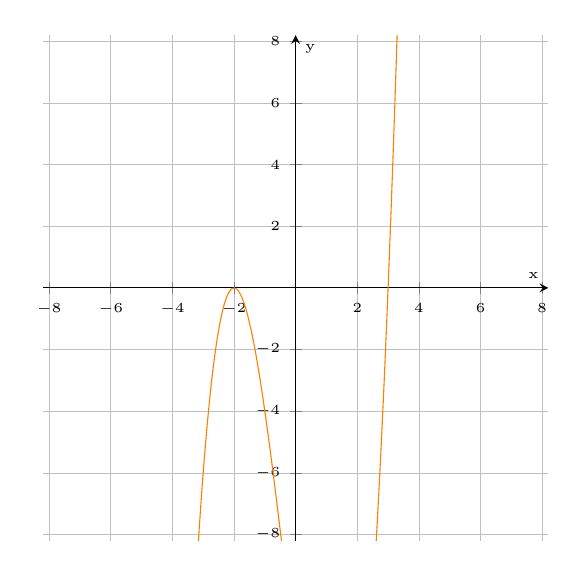
\begin{tikzpicture}
				\begin{axis}[
						xmin=-8.2, xmax=8.2,
						ymin=-8.2, ymax=8.2,
						height=8cm,
						width=8cm,
						grid=both,
						axis lines=middle,
						grid style={line width=.1pt, draw=gray!20},
						major grid style={line width=.2pt,draw=gray!50},
						ticklabel style={font=\tiny},
						xlabel style={font=\tiny},
						ylabel style={font=\tiny},
						xlabel={x}, ylabel={y}
					]
					\draw [orange, smooth, samples=100, domain=-4:4] plot
					(\x, {pow(\x, 3) + pow(\x,2) - 8 * \x - 12});
				\end{axis}
			\end{tikzpicture}
			\caption{Skizze}
		\end{figure}
	\end{loesung}
\end{uebung}
